%%%%%%%%%%%%%%%%%%% EJERCICIO 1 %%%%%%

%\newpage %USAR SOLO SI EL SOLUCIÓN QUEDA SOLO Y ES NECESARIO BAJARLO A LA SIGUIENTE PAGINA

%La tabla ira centrada
\begin{center}
  \renewcommand{\arraystretch}{1.5}% Margenes de las celdas
  %Creación de la cuadricula de 3 columnas
  \begin{flushleft}\textbf{A.2} \end{flushleft}
  \begin{longtable}[H]{|C{0.3\linewidth}|C{0.3\linewidth}|C{0.3\linewidth}|}
    %Creamos una linea horizontal
    \hline
    %Definimos el color de la primera fila
    \rowcolor[HTML]{FFB183}
    %%%%% INICIO ASIGNACIÓN FECHA FOCAL %%%%%%%
    %%%%%%%%%% INICIO TITULO
    %Lo que se hace aquí es mezclar las 3 columnas en una sola
    \multicolumn{3}{|c|}{\cellcolor[HTML]{FFB183}\textbf{1. Asignación período focal}}  \\ \hline
    %%%%%%%%%% FIN TITULO
    %%%%% INICIO DECLARACIÓN DE VARIABLES %%%%%%%
    \multicolumn{3}{|c|}{$pf = 4ptv$} \\ \hline
    %%%%%%%%%% INICIO TITULO
    %Lo que se hace aquí es mezclar las 3 columnas en una sola
    \multicolumn{3}{|c|}{\cellcolor[HTML]{FFB183}\textbf{2. Declaración de variables}}  \\ \hline
    %%%%%%%%%% FIN TITULO
    %%%%%%%%%% INICIO DE MATEMÁTICAS
    %Cada & hace referencia al paso de la siguiente columna
    
    $P =  200{.}000 COP$  & $i = 10\%\textit{ ptv} $  & $I= ? COP$   \\
      & $n=\frac{360 \textit{días}}{90 \textit{días}} =4 ptv$ & $F= ? COP$
    \\\hline

    %%%%%%%%%% FIN DE MATEMÁTICAS
    %%%%% FIN DECLARACIÓN DE VARIABLES

    %%%%% INICIO FLUJO DE CAJA
    \rowcolor[HTML]{FFB183}
    \multicolumn{3}{|c|}{\cellcolor[HTML]{FFB183}\textbf{3. Diagrama de flujo de caja}}                                                                          \\ \hline
    %Mezclamos 3 columnas y pondremos el dibujo
    %%%%%%%%%%%%% INSERCIÓN DE LA IMAGEN
    %Deberán descargar las imágenes respectivas del drive y pegarlas en la carpeta
    %n_capitulo/img/ejemplos/1/capitulo1ejemplo1.pdf  (el /1/ es el numero del ejemplo)
    \multicolumn{3}{|c|}{ 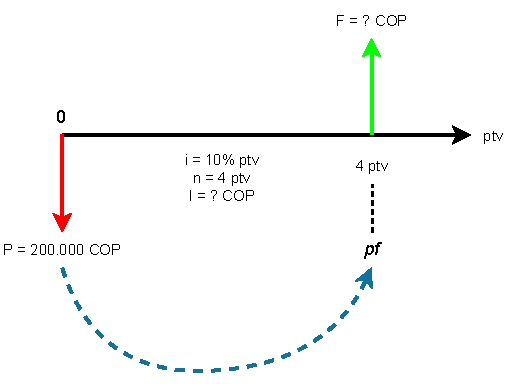
\includegraphics[trim=-5 -5 -5 -5 , scale=1]{2_Capitulo/ejemplos/1/Capitulo2Ejercicio1a2_v2.pdf} }                                         \\ \hline
    %%%%%%%%%%%%% FIN INSERCIÓN DE IMAGEN
    %%%%%FIN FLUJO DE CAJA

    %%%%% INICIO DECLARACIÓN FORMULAS
    %%%%%%%%%%% INICIO TITULO
    \rowcolor[HTML]{FFB183}
    \multicolumn{3}{|c|}{\cellcolor[HTML]{FFB183}\textbf{4. Declaración de fórmulas}}                                                                            \\ \hline
    %%%%%%%%%%% FIN TITULO
    %%%%%%%%%%% INICIO MATEMÁTICAS

    $I = Pin\hspace{0.3cm} \textit{Interés monetario simple}$ & \multicolumn{2}{c|}{$F = P + I \hspace{0.3cm} \textit{Valor futuro}$}                            \\ \hline
    %%%%%%%%%% FIN MATEMÁTICAS
    %%%%%% INICIO DESARROLLO MATEMÁTICO
    \rowcolor[HTML]{FFB183}
    %%%%%%%%%%INICIO TITULO
    \multicolumn{3}{|c|}{\cellcolor[HTML]{FFB183}\textbf{5. Desarrollo matemático}}                                                                              \\ \hline
    %%%%%%%%%% FIN TITULO
    %%%%%%%%%% INICIO MATEMÁTICAS
    $n=4ptv$                                                  & \multicolumn{2}{c|}{}                                                                            \\ $I_{1}= 200{.}000$ COP$\cdot0.1\cdot1$ & \multicolumn{2}{c|}{$F =  200{.}000$ COP + $20{.}000$ COP + $22{.}000$ COP}  \\ $I_{1}=  20{.}000$ COP & \multicolumn{2}{c|}{$+ 24{.}200$ COP + $26{.}620$ COP}  \\
    $I_{2}= 220{.}000\cdot0.1\cdot1$ COP   & \multicolumn{2}{c|}{$F= P+I$} \\
    $I_{2}= 22{.}000$ COP                  & \multicolumn{2}{c|}{$F=200{.}000$ COP$+92{.}820$ COP}   \\
    $I_{3}= 242{.}000\cdot0.1\cdot1$ COP   & \multicolumn{2}{c|}{$F= 292{.}820$ COP}                \\
    $I_{3}= 24{.}200$ COP                  & \multicolumn{2}{c|}{}                                                           \\
    $I_{4}= 266{.}200\cdot0.1\cdot1$ COP   & \multicolumn{2}{c|}{}                                                                            \\
    $I_{4}= 26{.}620$ COP                  & \multicolumn{2}{c|}{}                                                                            \\
    $I= 20{.}000 COP + 22{.}000 COP + 24{.}200 COP + 26{.}620 COP$& \multicolumn{2}{c|}{}                                        \\
    $I= 92{.}820$ COP                      & \multicolumn{2}{c|}{}
    
    \\ \hline
    %%%%%%%%%% FIN MATEMÁTICAS
    %%%%%% FIN DESARROLLO MATEMÁTICO
    %%%%%% INICIO RESPUESTA
    \rowcolor[HTML]{FFB183}
    %%%%%%%%%%INICIO TITULO
    \multicolumn{3}{|c|}{\cellcolor[HTML]{FFB183}\textbf{6. Respuesta}}                                                                                          \\ \hline
    %%%%%%%%%% FIN TITULO
    %%%%%%%%%% INICIO RESPUESTA MATEMÁTICA
    $I= 92{.}820 COP$                                         &
    \multicolumn{2}{c|}{$F= 292{.}820 COP$
    }                                                                                                                                                            \\ \hline
    %%%%%%%%%% FIN MATEMÁTICAS
    %%%%%% FIN RESPUESTA
  \end{longtable}
  %Se crean dos lineas en blanco para que no quede el siguiente texto tan pegado
  %\newline \newline %USARLO SI CREES QUE ES NECESARIO
\end{center}
%%%%%%%%%%%%%%%%%%%%%%%%%%FIN EJERCICIO 1 %%%%%%%%%%%%%%%%%%%%%%%%%%%

